\subsection{Architettura delle API}
Ho continuato quindi il mio studio passando all'analisi dell'architettura delle \gls{api}, che come ho accennato nel capitolo 
\ref{chap:vincoli tec} sono sviluppate utilizzando il \textit{framework} ASP.NET Core. 
Il \textit{back-end} di {\movi} si trova in una \textit{repository} BitBucket a sè stante rispetto al \textit{front-end} per consentire 
una gestione più efficiente e modulare del progetto. Questo permette: 
\begin{itemize}
    \item \textbf{Manutenibilità}: facilita la manutenzione e l'aggiornamento di ciascuna componente senza impattare l'altra;
    \item \textbf{Flessibilità}: permette l'utilizzo di tecnologie e \textit{framework} diversi per \textit{back-end} e 
          \textit{front-end}, ottimizzando ciascuno per il proprio scopo e facilitando eventuali cambiamenti di tecnologie futuri;
    \item \textbf{Versionamento}: consente una versionamento separato per le due parti dell'applicazione e semplifica il 
          tracciamento delle modifiche del codice;
    \item \textbf{Riutilizzo del codice}: Facilita il riutilizzo del \textit{back-end} per diverse interfacce o applicazioni.
\end{itemize}

\begin{figure}[H]
    \centering
    %\hspace{-3.25cm} % Sposta la figura a sinistra di n cm
    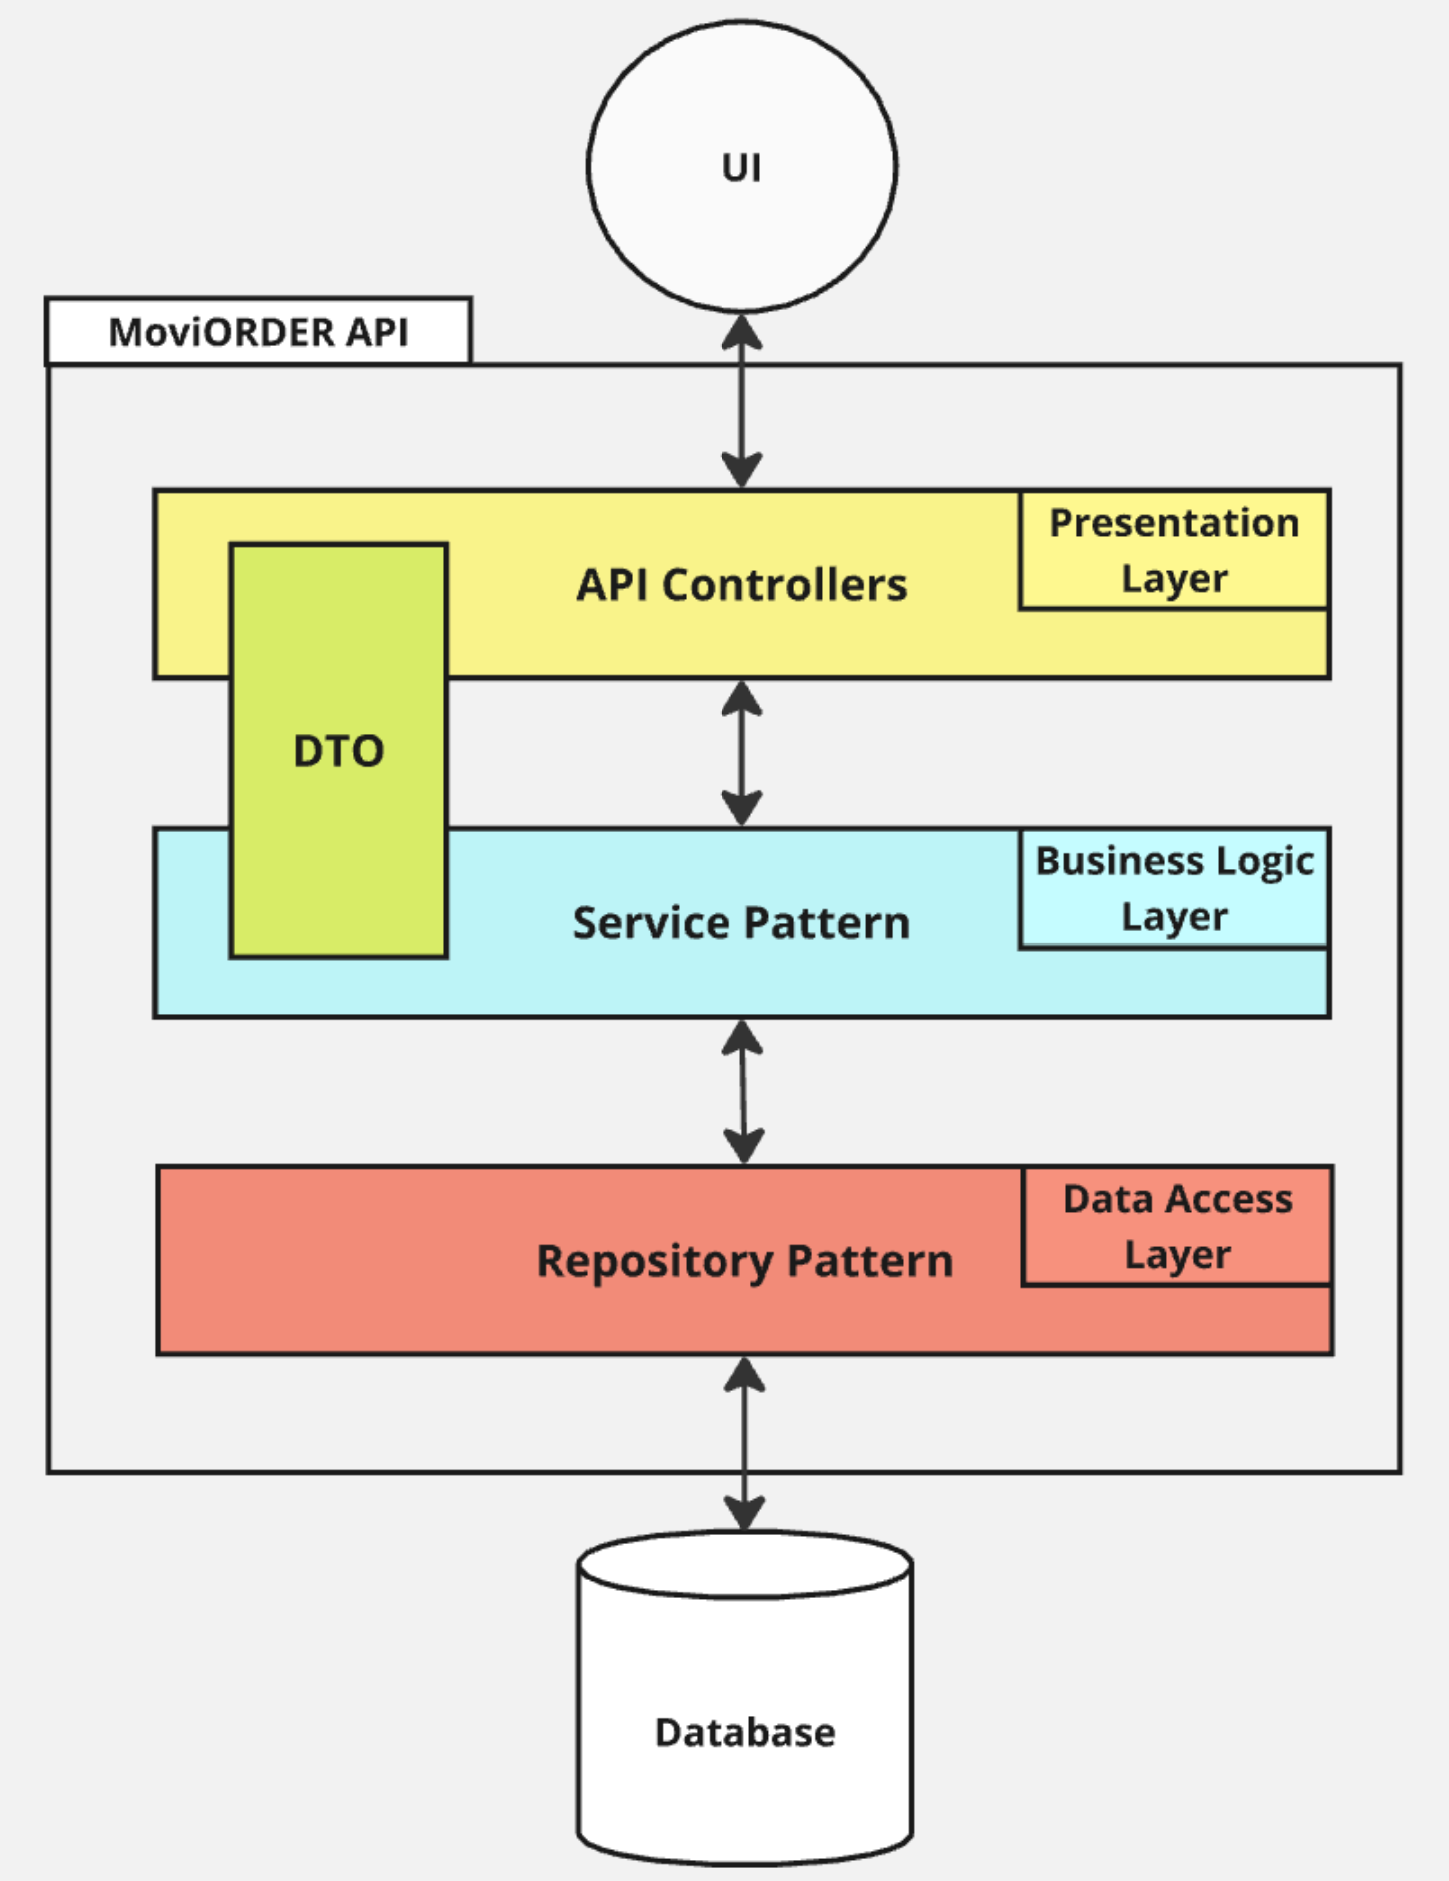
\includegraphics[width=0.6\textwidth]{img/repository-service.png}
    \caption{Architettura API.}
    \label{fig:repository-service}
\end{figure}

Le \gls{api} di {\movi} adottano un'architettura a livelli, combinando il \textit{Pattern Repository} e il \textit{Pattern Service}, 
come mostra la figura \ref{fig:repository-service}, garantendo scalabilità, manutenibilità e sicurezza.
Questa architettura stratifica il codice in livelli di astrazione crescente, 
partendo dallo strato più "concreto" in diretta interazione con il \textit{database}, fino a quello più 
"astratto" che si interfaccia con il \textit{front-end}.